\newpage\thispagestyle{hl}
\hlbanner{The whole book}{}{At a glance}
\hlsection{What the book is}
\begin{hlquote}This book describes how a reduced-order modelling package, \rom{}, is built on top of a finite element package, \fea{}, for the analysis of structures, and checks, one claim at a time, that the two packages do what is said of them.\end{hlquote}
It is written for readers who already know the finite element method and the idea of model reduction, and who want to see how the two meet in working code. Every listing was run, and every number in the text is generated by a script and enters the book as a macro.
\hlsection{The two packages and how they meet}
\begin{center}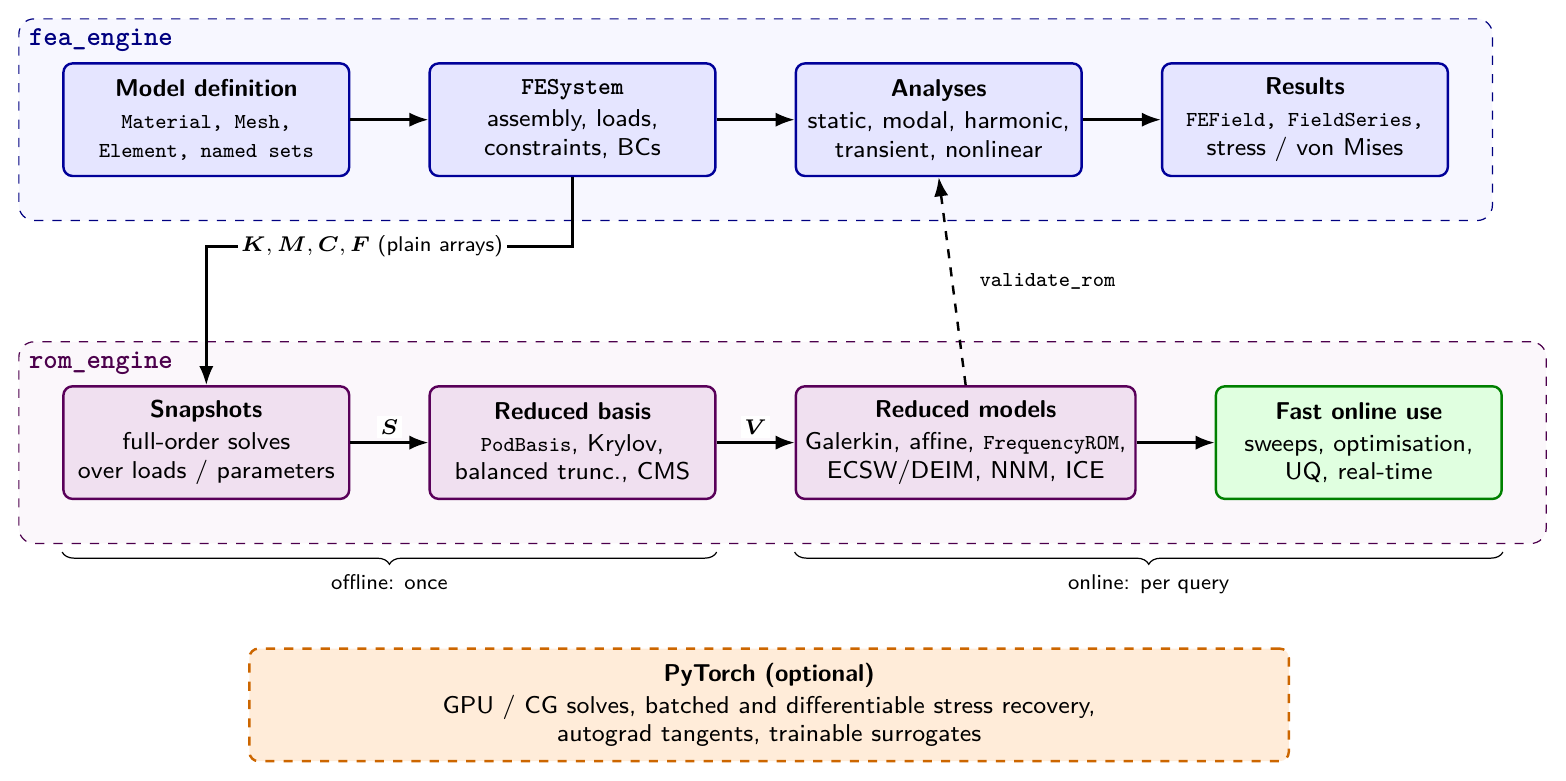
\includegraphics[width=\linewidth]{figures/architecture.png}\end{center}
{\small\color{hlgrey}\textbf{Figure.} \fea{} produces the matrices and the full-order solutions; \rom{} works on plain arrays, never imports \fea{}, and returns reduced models for fast online use.}
\hlsection{Four parts, fourteen chapters}
{\small\begin{tabularx}{\linewidth}{@{}p{0.27\linewidth}>{\raggedright\arraybackslash}p{0.1\linewidth}X@{}}
\textsf{\textbf{\color{hlnavy}Architecture}} & Ch.\ 1--2 & the design of the engine, and meshes that are checked rather than assumed \\[3pt]
\textsf{\textbf{\color{hlnavy}Full-order physics}} & Ch.\ 3--7 & elements and locking, dynamics, nonlinearity, batched assembly, exact contact \\[3pt]
\textsf{\textbf{\color{hlnavy}Reduced-order modelling}} & Ch.\ 8--13 & POD--Galerkin, balanced truncation, Krylov and SOAR, frequency-domain and greedy, substructuring, non-intrusive and nonlinear, hyper-reduction and contact \\[3pt]
\textsf{\textbf{\color{hlnavy}Verification}} & Ch.\ 14 & what ``verified'' means, nine reproduction studies, an integrated pipeline \\
\end{tabularx}}
{\small Four appendices follow: differentiable assembly, conventions and tolerances, a glossary, and a map from chapters to the package tests that cover them.}

\newpage\thispagestyle{hl}
\hlbanner{The whole book}{}{How it is built}
\hlsection{Six levels of evidence}
\hlfig{\hltikz{ch14_pyramid}}{Each number in the book sits on one of six levels, from a unit test to an integrated run. The references are never the code under test.}
\hlsection{Every chapter has the same layout}
An opening box and a concrete problem; the mathematical structure; the implementation in the packages, with pseudocode, cost and failure modes; a Verification section; a box of limits; a summary; exercises of three kinds (derivation, implementation, interpretation). Short boxes inside the text define terms where they are first needed.
\hlsection{Nine published studies, rebuilt from the packages}
{\small\begin{tabularx}{\linewidth}{@{}>{\raggedright\arraybackslash}p{0.5\linewidth}X@{}}
Multi-fidelity surrogate ROM (He, 2023) & reproduced; one reference fails at large amplitude \\
Hybrid modal ROM (Yang, 2019) & reproduced on a panel; open defect on a plate \\
Implicit condensation and expansion (Hollkamp, 2008) & statics reproduced; dynamics not \\
Loewner identification, plate in air and water (Liu, 2026) & method reproduced against the author's truth model \\
Frequency-domain PINN (Liang, 2024) & inverse problem reproduced; forward field not \\
Hybrid hyper-reduction for contact (Fauqu\'e, 2018) & accuracy reproduced; speed-up not \\
Assembly reduction with contact (Nikiema, 2026) & qualitative result reproduced \\
Projection-based contact reduction (Balajewicz, 2016) & reproduced \\
FE-ROM-informed neural operator (Yang, 2025) & single tones reproduced; generalisation not \\
\end{tabularx}}
{\small The failures are reported with the successes.}

\newpage\thispagestyle{hl}
\hlbanner{For reviewers}{}{Request the full draft}
\hlsection{What you would receive}
\begin{itemize}\setlength\itemsep{3pt}
\item the full draft of the book (about 330 pages, with listings, figures and exercises);
\item the pinned release of the two packages that every listing and number refers to, and the scripts that generate the numbers;
\item a short reviewer guide with the questions below.
\end{itemize}
\hlsection{What I would value your view on}
\begin{enumerate}\setlength\itemsep{3pt}
\item Are the definitions accurate, and at the right depth for a reader who knows finite elements and model reduction in outline?
\item Is the order of the chapters and the layout of a chapter helpful? Which topic is missing, and which is too long?
\item Do the verification sections convince you of the claims they support, and are the limits stated fairly?
\item Would you use this book alongside a course or a research project, and for which reader?
\end{enumerate}
\hlsection{How to proceed}
\begin{enumerate}\setlength\itemsep{3pt}
\item Reply with your name, affiliation and the review terms on the next page marked as accepted.
\item You receive the full draft with a download link that I can withdraw.
\item Comments are welcome in any form; a first pass of two to four weeks is ideal.
\end{enumerate}
\hlsection{Contact}
Abhijeet Kumar \quad \url{https://www.linkedin.com/in/abhijeet-kumar-phd-a689b429} \quad \url{https://github.com/abhi2k16} \quad [contact e-mail]

\newpage\thispagestyle{hl}
\hlbanner{For reviewers}{}{Review terms (draft)}
\begin{hllimit}\small This page is a draft for legal review. It is a template, not legal advice, and the bracketed items are to be completed before it is used.\end{hllimit}
{\small
\begin{enumerate}\setlength\itemsep{3pt}
\item \textbf{Parties and purpose.} Abhijeet Kumar (the Author) provides the full draft of the book \emph{Implementing Reduced-Order Modeling In Computational Mechanics} (the Draft) to the person named in the acceptance (the Reviewer) only to obtain the Reviewer's opinion on it.
\item \textbf{Confidentiality.} The Reviewer keeps the Draft confidential and does not copy, forward, post, publish or share it or any part of it, and does not use it for any purpose other than the review. The Reviewer does not submit the Draft, or text from it, to any machine-learning or text-generation service.
\item \textbf{Ownership.} The Draft, its text, figures and listings remain the property of the Author. The code of the two packages is available under the MIT license stated in the Draft; this does not extend to the text or the figures of the book.
\item \textbf{Feedback.} The Reviewer's comments may be used by the Author freely, without obligation, to improve the book. The Author will acknowledge the Reviewer by name in the book only if the Reviewer agrees in writing.
\item \textbf{No warranty.} The Draft is a work in progress and is provided as it is. It may contain errors, and no warranty of accuracy or fitness for any purpose is given.
\item \textbf{Term.} The obligations of confidentiality continue for [24 months] from the date of acceptance, or until the Draft is published, whichever is earlier. On request the Reviewer deletes all copies of the Draft.
\item \textbf{Law.} These terms are governed by the law of [jurisdiction]; the courts of [place] have jurisdiction.
\end{enumerate}
\vspace{4pt}\noindent\textbf{Acceptance.} Name: \rule{5cm}{0.3pt}\quad Affiliation: \rule{5cm}{0.3pt}\quad Date: \rule{3cm}{0.3pt}\\[6pt]
A reply by e-mail stating ``I accept the review terms'' with the Reviewer's name and affiliation is sufficient.}
